\documentclass{article}\usepackage[]{graphicx}\usepackage[]{color}
% maxwidth is the original width if it is less than linewidth
% otherwise use linewidth (to make sure the graphics do not exceed the margin)
\makeatletter
\def\maxwidth{ %
  \ifdim\Gin@nat@width>\linewidth
    \linewidth
  \else
    \Gin@nat@width
  \fi
}
\makeatother

\definecolor{fgcolor}{rgb}{0.345, 0.345, 0.345}
\newcommand{\hlnum}[1]{\textcolor[rgb]{0.686,0.059,0.569}{#1}}%
\newcommand{\hlstr}[1]{\textcolor[rgb]{0.192,0.494,0.8}{#1}}%
\newcommand{\hlcom}[1]{\textcolor[rgb]{0.678,0.584,0.686}{\textit{#1}}}%
\newcommand{\hlopt}[1]{\textcolor[rgb]{0,0,0}{#1}}%
\newcommand{\hlstd}[1]{\textcolor[rgb]{0.345,0.345,0.345}{#1}}%
\newcommand{\hlkwa}[1]{\textcolor[rgb]{0.161,0.373,0.58}{\textbf{#1}}}%
\newcommand{\hlkwb}[1]{\textcolor[rgb]{0.69,0.353,0.396}{#1}}%
\newcommand{\hlkwc}[1]{\textcolor[rgb]{0.333,0.667,0.333}{#1}}%
\newcommand{\hlkwd}[1]{\textcolor[rgb]{0.737,0.353,0.396}{\textbf{#1}}}%
\let\hlipl\hlkwb

\usepackage{framed}
\makeatletter
\newenvironment{kframe}{%
 \def\at@end@of@kframe{}%
 \ifinner\ifhmode%
  \def\at@end@of@kframe{\end{minipage}}%
  \begin{minipage}{\columnwidth}%
 \fi\fi%
 \def\FrameCommand##1{\hskip\@totalleftmargin \hskip-\fboxsep
 \colorbox{shadecolor}{##1}\hskip-\fboxsep
     % There is no \\@totalrightmargin, so:
     \hskip-\linewidth \hskip-\@totalleftmargin \hskip\columnwidth}%
 \MakeFramed {\advance\hsize-\width
   \@totalleftmargin\z@ \linewidth\hsize
   \@setminipage}}%
 {\par\unskip\endMakeFramed%
 \at@end@of@kframe}
\makeatother

\definecolor{shadecolor}{rgb}{.97, .97, .97}
\definecolor{messagecolor}{rgb}{0, 0, 0}
\definecolor{warningcolor}{rgb}{1, 0, 1}
\definecolor{errorcolor}{rgb}{1, 0, 0}
\newenvironment{knitrout}{}{} % an empty environment to be redefined in TeX

\usepackage{alltt}
\usepackage{amsmath} %This allows me to use the align functionality.
                     %If you find yourself trying to replicate
                     %something you found online, ensure you're
                     %loading the necessary packages!
\usepackage{amsfonts}%Math font
\usepackage{graphicx}%For including graphics
\usepackage{hyperref}%For Hyperlinks
\usepackage{hyperref}
\hypersetup{colorlinks = true,citecolor=black}
\usepackage{natbib}        %For the bibliography
\bibliographystyle{apalike}%For the bibliography
\usepackage[margin=0.50in]{geometry}
\usepackage{float}
\usepackage{multicol}

%fix for figures
\usepackage{caption}
\newenvironment{Figure}
  {\par\medskip\noindent\minipage{\linewidth}}
  {\endminipage\par\medskip}
\IfFileExists{upquote.sty}{\usepackage{upquote}}{}
\begin{document}

\vspace{-1in}
\title{Final Exam for MATH 354 -- Data Analysis I \\
Submission and Formatting Instructions}

\author{
  First Author \\
  Affiliation  \\
  Department  \\
  {\tt email@domain}
}

\date{}

\maketitle

\begin{multicols}{2}
\begin{abstract}
This document provides a basic template for the 2-page extended abstract and some submission guidelines.
\end{abstract}

{\bf Keywords:} Optional, Yet Potentially, Helpful

%%% R code for in-paper reference



%%% Write up!
\section{Introduction}
\subsection{What we've done}
On the midterm exam, you should have been able to show that wellbeing measures increased, and illbeing measures decreased. The effects were small, but several of them were significant. I don't know about you, but that's enough for me to want to play with some dogs.

We hadn't discussed regression techniques as of the midterm, so we could not do the analysis while ``controlling" for other variables; e.g., gender, age, whether they have pets at home, etc. For the final analysis, we take another step forward!

\subsection{Prompt}
The prompt for this exam is based on my joint work with Erin Cooley (Colgate), Jazmin Brown-Iannuzzi (UVA), Ryan Lei (Haverford), and Lauren Philbrook (Colgate). Our most recent research explored how beliefs about White poverty play a role in forming White Americans' policy attitudes.

The data consists of observations on 837 non-Hispanic Black and White Americans who were not receiveing welfare. We measured their beliefs that White people are poor; their beliefs that Black people are poor; their perception that welfare recipients are hardworking; their general support for welfare policy; and information about the race, political affiliation, income, and education of participants.

The study results support the hypothesis that beliefs White people are poor predict beliefs that White people benefit from welfare. This belief mediates a greater tendency to humanize welfare recipients, with downstream consequences for greater support for agentic welfare policy (i.e., cash assistance). Further, we found that these processes may be motivated: White Americans high in zero-sum beliefs, the beliefs that one person's or group's loss is anothers gain, showed a stronger association between beliefs that White people benefit from welfare and the humanization of welfare recipients.

Use regression models and posthoc evaluations to evaluate the data from Study 1 (described below). Ensure that the statistical procedures you selected are appropriate for these data. You will note that this template is just two pages long, not including bibliograpy and apendix -- this ensures that you can determine what is necessary for succinctly, but fully, answering this question. 

\subsection{Template}
This template is based on the SDSS conference template, which is based the template for the annual conference of the Association for Computational Linguistics (ACL), whose template includes the following paragraph of credits:
\begin{quotation}
\small % Okay to use \small inside quotation environment ONLY
This document has been adapted from the instructions for earlier ACL proceedings, including those for ACL-2012 by Maggie Li and Michael White, those from ACL-2010 by Jing-Shing Chang and Philipp Koehn, those for ACL-2008 by Johanna D. Moore, Simone Teufel, James Allan, and Sadaoki Furui, those for ACL-2005 by Hwee Tou Ng and Kemal Oflazer, those for ACL-2002 by Eugene Charniak and Dekang Lin, and earlier ACL and EACL formats. Those versions were written by several people, including John Chen, Henry S. Thompson and Donald Walker. Additional elements were taken from the formatting instructions of the {\em International Joint Conference on Artificial Intelligence}.
\end{quotation}  
The goal of this two-page template is to emphasize extracting what's essential.

In preparing your final analysis I strongly encourage using the same four section headings seen here, namely, Introduction, Methods, Data (or Results), and Discussion (or Conclusions). Use of subsections is at your discretion.

You submission \emph{must} be two-pages long, with the option of a 1 page appendix showing your most important code chunks.

\subsection{Citations}
In \LaTeX, please use the Bib\TeX{} bibliography style, as demonstrated by this example document. Review the paragraph below in the .RnW file; itshows how the LaTeX and 
Bib\TeX{} code work together to generate the citations.

Citations within the text appear in parentheses as \citep{Nussbaum2018} or, if the author's name appears in the text itself, as \cite{Nussbaum2018}.  Treat double authors as in \cite{Wasserstein2016}. Collapse multiple citations as in \citep{Nussbaum2018,Wasserstein2016}. As alluded to above, full citations should not be used as sentence constituents.  For instance, instead of
\begin{quote}
  ``\cite{Arbuthnot1710} derived the earliest $p$-value ...''
\end{quote}
use
\begin{quote}
``\cite{Arbuthnot1710} derived the earliest $p$-value ...''.
\end{quote}
Please make references complete, presentable, and consistent. When using Bib\TeX{}, protect capital letters of names and abbreviations in titles, as in \{B\}ayesian or \{EM\} algorithm, in your .bib file.  For an example, notice that the ``FDA'' in the title of \cite{LaVange2019} is typed as \verb+{FDA}+ in the .bib file or else it would be incorrectly shown as ``fda'' in the references section.

The \LaTeX{} and Bib\TeX{} style files provided roughly fit the American Psychological Association format, allowing regular citations, short citations and multiple citations as described above.

\subsection{Graphics and Tables}
Place figures and tables in the paper near where they are first discussed, rather than at the end. 

\begin{Figure}
\begin{center}
%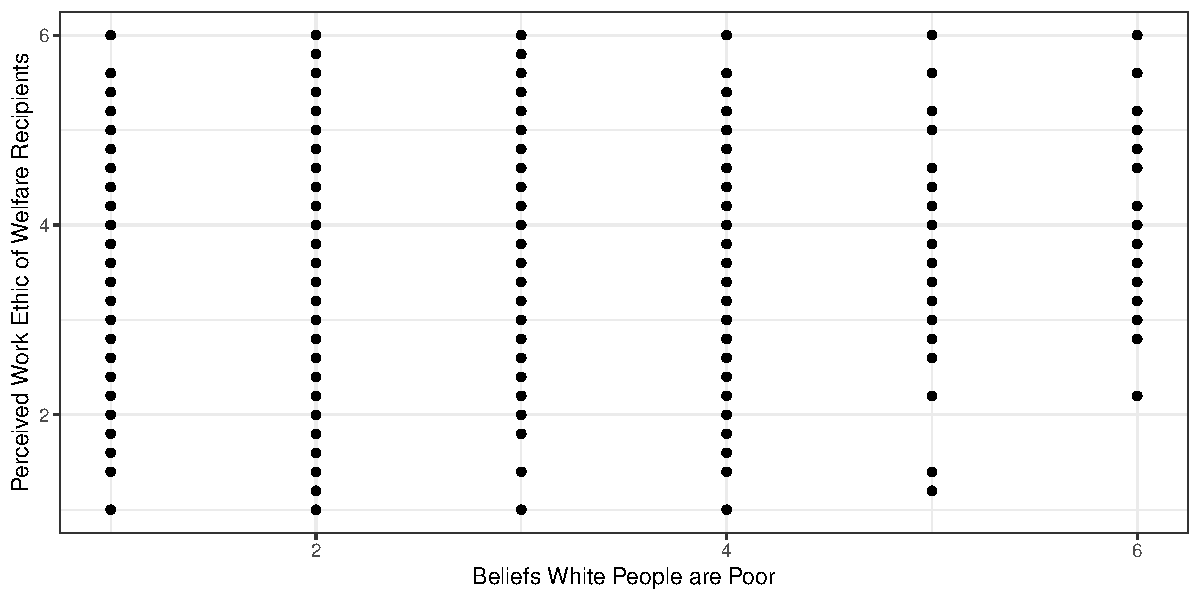
\includegraphics[width=\columnwidth]{figure/workethic.pdf} %call created figure
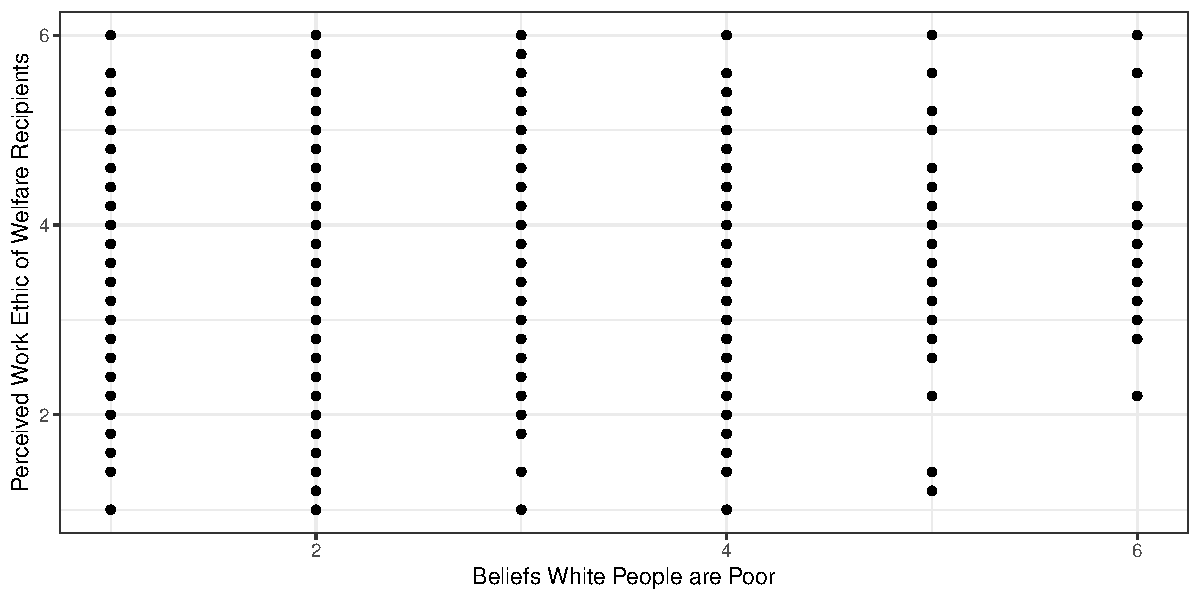
\includegraphics[width=\linewidth]{figure/workethic.pdf} %call created figure
\captionof{figure}{An example plot using the data.}
\label{bayespic}
\end{center}
\end{Figure}

\section{Methods}
You may use this prompt to help build your introduction and methods sections. You want to provide some essential information about what you're addressing
and where the data came from.

\section{Data/Results}
\subsection{Models}
Fit the following models to help answer the questions of the researcher with our new-found tools.

\subsubsection{Work Ethic}
In Study 1 of the paper, we build a regression model for the perceived work ethic of welfare recipients (\texttt{HardworkingWelf}) based on beliefs White people are poor (\texttt{Wpoor}), race of the participant (\texttt{PsWhite}), and their interaction. Create and interpret this model in the context of the question. Ensure to control for education (\texttt{edu}), income (\texttt{income}), political affiliation (\texttt{Democrat}), and beliefs Black people are poor (\texttt{Bpoor}).

\subsubsection{A Challenge}
A main goal of this course is to give you a solid foundation. It's less important to memorize every detail of the course than it is to learn how to approach a data problem. I hope that you've learned enough to come across something new, and tackle it with the help of documentation and vignettes. As a challenge, you might want to consider mediation analysis, which quantifies the effect of one independent variable ``through" another. See the \texttt{mediation} package for \texttt{R} \citep{mediation1, mediation2}.

To demonstrate that you've learned enough to pick up new modeling techniques, try using mediation to explore Study 1. Specifically, does the race of the participant moderate the effect of beliefs White people are poor through the perceived work ethic of welfare recipients (the possible mediator)?

\subsubsection{An Optional Bonus}
Locate data documenting the percentage of people below the poverty line who are White by zip code and add that as a variable in the data set. Check if this variable (percentage of white people in poverty in the participant's location) predicts the degree of beliefs that White people are poor. In other words, are these race/class stereotypes shaped by sensitivity to the racial distribution of poverty in one's area?

\section{Discussion/Conclusions}
Discuss the results of your analyses here. This is where you tie all of your work together into a nice, succinct summary.

\subsection{Submissions}
This part of the final is "self-scheduled." I know y'all have projects and finals coming up. It is expected that the final will be submitted by the end of finals week, Friday, December 17	by 5p. I will not accept late submissions.

\subsection{Short Answer Part}
The short answer questions for the final will look similar to the short answer question on the midterm. While the data analysis aims to measure ``what you can do," the short answer questions aim to measure ``what you're walking around with." These questions will be available to complete as a quiz on Moodle between 3:00p and 5:00p on December 13th. This will take 35 minutes. Keep in mind these are meant to be questions about ``big picture" understanding rather than small technicalities.

%%%%%%%%%%%%%%%%%%%%%%%%%%%%%%%%%%%%%%%%%%%%%%%%%%%%%%%%%%%%%%%%%%%%%%%%%%%%%%%%
% Bibliography
%%%%%%%%%%%%%%%%%%%%%%%%%%%%%%%%%%%%%%%%%%%%%%%%%%%%%%%%%%%%%%%%%%%%%%%%%%%%%%%%
\newpage
\bibliography{final.bib}
\end{multicols}

%%%%%%%%%%%%%%%%%%%%%%%%%%%%%%%%%%%%%%%%%%%%%%%%%%%%%%%%%%%%%%%%%%%%%%%%%%%%%%%%
% Appendix
%%%%%%%%%%%%%%%%%%%%%%%%%%%%%%%%%%%%%%%%%%%%%%%%%%%%%%%%%%%%%%%%%%%%%%%%%%%%%%%%
\newpage
\onecolumn
\section{Appendix}
\begin{scriptsize}
Below are examples of how to incorporate your code.\\\vspace{1em}

Loaded Data.
\begin{knitrout}
\definecolor{shadecolor}{rgb}{0.969, 0.969, 0.969}\color{fgcolor}\begin{kframe}
\begin{alltt}
\hlkwd{library}\hlstd{(tidyverse,}\hlkwc{quietly} \hlstd{= T)}
\hlkwd{suppressMessages}\hlstd{(dat} \hlkwb{<-} \hlkwd{read_csv}\hlstd{(}\hlstr{"final.csv"}\hlstd{,} \hlkwc{na}\hlstd{=}\hlstr{"#NULL!"}\hlstd{))} \hlcom{# Study 1}
\end{alltt}
\end{kframe}
\end{knitrout}
Plot plot.
\begin{knitrout}
\definecolor{shadecolor}{rgb}{0.969, 0.969, 0.969}\color{fgcolor}\begin{kframe}
\begin{alltt}
\hlkwd{pdf}\hlstd{(}\hlstr{"figure/workethic.pdf"}\hlstd{,}\hlkwc{width}\hlstd{=}\hlnum{8}\hlstd{,} \hlkwc{height}\hlstd{=}\hlnum{4}\hlstd{)}  \hlcom{#save ggplot to a pdf}
\hlkwd{ggplot}\hlstd{(}\hlkwc{data}\hlstd{=dat,}\hlkwd{aes}\hlstd{(}\hlkwc{x}\hlstd{=Wpoor,} \hlkwc{y}\hlstd{=HardworkingWelf))}\hlopt{+}
  \hlkwd{geom_point}\hlstd{()}\hlopt{+}
  \hlkwd{theme_bw}\hlstd{()}\hlopt{+}
  \hlkwd{xlab}\hlstd{(}\hlstr{"Beliefs White People are Poor"}\hlstd{)}\hlopt{+}
  \hlkwd{ylab}\hlstd{(}\hlstr{"Perceived Work Ethic of Welfare Recipients"}\hlstd{)}
\hlkwd{dev.off}\hlstd{()}
\end{alltt}
\end{kframe}
\end{knitrout}

\end{scriptsize}
\end{document}
